\chapter{Development Plan \& Problem Exploration}\label{chp:Problems}
This chapter will investigate how the protocol can be perceived mathematically as a graph, and how it can be divided into simpler subproblems which can be solved iteratively.

The requirements stated in the previous chapter, can be modelled as a graph problem where a weighted directed graph $G = (V, E)$ describes the network. 
The vertices, $V$, are the devices and the edges, $E$, are the communication paths between the devices. 
The weight, $W(v_1, v_2)$, is the probability of a message from $v_1$ successfully being received by $v_2$.
An example of this can be seen on \myref{fig:network}.
For this project only networks which can be depicted as completely or strongly connected graphs will be considered, to ensure that all devices will have the possibility to exchange information with every other device.
In \myref{fig:examplenetworkgraphs} the two different network types are modelled as graphs; \myref{fig:network} is an example of a strongly connected network which can be described as: $E \subseteq V \times ]0,1] \times V$ where for any $v_i, v_j$ there exists a path from $v_i$ to $v_j$ with the reliability $r$ which is a number in the range $]0,1]$.

\begin{figure}[h]
    \begin{subfigure}{0.5\linewidth}
        \centering
        \begin{tikzpicture} [
        node distance = 1 cm, 
        vertex/.style = {circle, draw, fill=blue!10}, 
        label/.style={fill=white}
    ]

    \node[draw=none](0){};
    \node[vertex, left  = 2cm of 0]   (1) {$v_1$};
    \node[vertex, above =     of 0]   (2) {$v_2$};
    \node[vertex, right = 2cm of 0]   (3) {$v_3$};
    \node[vertex, below =     of 0]   (4) {$v_4$};
    
    \path[thick] (1) edge (2) edge (3) edge (4);
    \path[thick] (3) edge (2) edge (4);
    \path[thick] (2) edge (4);
\end{tikzpicture}  
        \caption{Completely connected network.}
        \label{fig:ccrcnetworkgraph}
    \end{subfigure}\hfill
    \begin{subfigure}{0.5\linewidth}
        \centering
        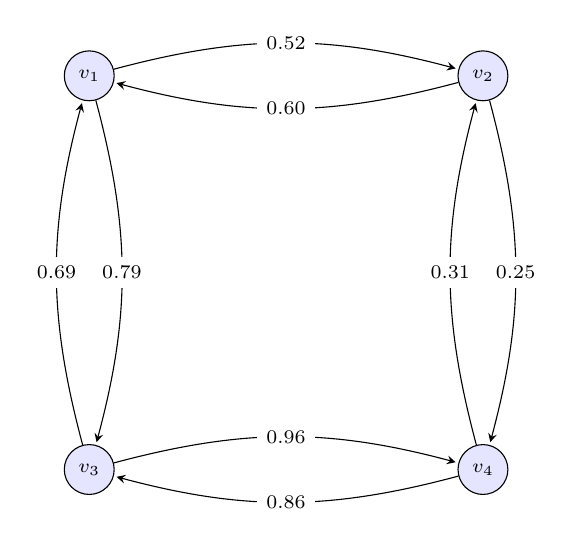
\begin{tikzpicture} [
        node distance = 5 cm, 
        font=\scriptsize, 
        vertex/.style = {circle, draw, fill=blue!10}, 
        edge/.style = {draw, -stealth, shorten >= 1pt},
        label/.style={fill=white}
    ]

    \node[vertex](1){$v_1$};
    \node[vertex, right of=1](2){$v_2$};
    \node[vertex, below of=1](3){$v_3$};
    \node[vertex, below of=2](4){$v_4$};
    
    \path[edge] (1) edge[bend left=15] node [label] {0.79} (3) edge[bend left=15] node [label] {0.52} (2);
    \path[edge] (2) edge[bend left=15] node [label] {0.25} (4) edge[bend left=15] node [label] {0.60} (1);
    \path[edge] (3) edge[bend left=15] node [label] {0.96} (4) edge[bend left=15] node [label] {0.69} (1);
    \path[edge] (4) edge[bend left=15] node [label] {0.31} (2) edge[bend left=15] node [label] {0.86} (3);;
    
\end{tikzpicture}
        \caption{Strongly connected unreliable network with probabilities.}
        \label{fig:network}
    \end{subfigure}
    \caption{Examples of networks modelled as graphs.}
    \label{fig:examplenetworkgraphs} 
\end{figure}

\noindent Creating a protocol for such a network as shown in \myref{fig:network} is a complex problem to solve and many issues will become apparent throughout analysis of the problem.
In order to simplify the problem some assumptions are made about the network.
%We assume that the devices will always be in range of each other; this means that all vertices on the graph have a non-zero edge between all other vertices on the graph.
During development of the system, the system could be set up to give \textasciitilde100 \% probability of successfully receiving the message, by wiring the Arduinos together instead of using radio communication; this gives more room to work on the baseline communication issues without having to consider the unreliability of the radio frequency modules.
As previously mentioned the networks can be set up as either completely connected graphs (as in \myref{fig:ccrcnetworkgraph}) or strongly connected graphs (as in \myref{fig:network}).
As a consequence of this, four sub problems will be considered and modelled as graphs:

\begin{description}[labelindent=\parindent,itemsep=2em]
    \item[\gls{ccrc}-problem:]   
    \begin{equation}
		\text{iff } \forall\, \{v_i, v_j\} \subset V: \, (v_i,r,v_j)\in E \mid r = 1    
    \end{equation}
    The \gls{ccrc}-problem describes a network where all vertices are directly connected with each other, creating a completely connected graph.
	All the weights of the edges in this graph are 1, which means that all transmissions will be received. 
    
    \item[\gls{ccuc}-problem:]
    \begin{equation}
		\text{iff } \forall\, \{v_i, v_j\} \subset V: \, (v_i,r,v_j)\in E \mid r \in (0, 1]
    \end{equation}
    The \gls{ccuc}-problem describes a completely connected graph however in this scenario there is not a guarrentee that the transmission will be received; all vertices are still in range of each-other. 
    
    \item[\gls{scrc}-problem:]
    \begin{equation}
		\begin{gathered}
			\text{iff } \forall\, \{v_i, v_j\} \subset V: \text{ there is a directed path from } v_i \text{ to } v_j\; \land \\ \forall\, (v_q, r, v_r) \in E : r = 1
		\end{gathered}  
    \end{equation}   
    The \gls{scrc}-problem describes a strongly connected network meaning at least one vertex does not have direct connections to all other verticies, i.e. there still exists a path from every vertex to every other vertex but at least one pair of vertices requires one or more mediating vertices. 
	In this example communication is once again reliable such that all transmissions will be received. 
    
    \item[\gls{scuc}-problem:]
    \begin{equation}
		\begin{gathered}
			\text{iff } \forall\, \{v_i, v_j\} \subset V: \text{ there is a directed path from } v_i \text{ to } v_j\; \land \\ \forall\, (v_q, r, v_r) \in E : r \in (0, 1]
		\end{gathered}  
    \end{equation}    
    The \gls{scuc}-problem describes the most realistic scenario, a strongly connected network with a chance of not receiving transmissions. 
\end{description}
\bigskip \noindent
The \gls{ccrc}-problem is is the obvious choice for the first iteration, since this is the simplest problem, which requires the least amount of design choices to be fulfilled.
The decision of which problem should follow \gls{ccrc}-solution, is however a more complex discussion.
One could argue for expanding into a still reliable but now only \acrlong{scrc}, as well as arguing for expanding into a unreliably but still \acrlong{ccuc}.
Therefor the chosen order will simply reflect our estimation of which problems will require the least amount of modification.

Another possibility would be to only split the sub problems into three, e.g. \gls{ccrc} $\rightarrow$ \gls{ccuc} $\rightarrow$ \gls{scuc}.
However we deem that a more optimal solution can be derived by working with the strongly connected problem followed by the unreliable problem and then combine the solutions to solve the \gls{scuc}-problem.

In addition to these four sub problems, some more practical problems will be abstracted away for in the first iteration.
An example of such a abstraction could be starting multiple devices at the same time.
Solutions to these practical problems will be implemented continually during the development. 
This approach increases the probability of having a working solution at the end of this project without over- or underestimating the workload. 
